\documentclass[a4paper]{article}
\newif\ifshowcode
\showcodetrue

\usepackage{latexsym}
\usepackage[portuges]{babel}
\usepackage{a4wide}
\usepackage[utf8]{inputenc}
\usepackage{graphicx}
\usepackage{graphics}
\usepackage{glossary}
\usepackage{algorithmic}
\usepackage{algorithm}
\usepackage{listings}
\usepackage[toc,page]{appendix}

\parindent=0pt
\parskip=2pt

\setlength{\oddsidemargin}{0in}
\setlength{\evensidemargin}{0in}
\setlength{\topmargin}{0in}
\addtolength{\topmargin}{-\headheight}
\addtolength{\topmargin}{-\headsep}
\setlength{\textheight}{8.9in}
\setlength{\textwidth}{6.5in}
\setlength{\marginparwidth}{0.5in}

%
% Report to Engineering Languages UCE
%
\title{\huge \bigskip
\begin{figure}[!ht]
\begin{flushright}

\includegraphics[width=0.2\textwidth]{./Images/um-eng.jpg} \vspace{1cm}
\end{flushright}
\end{figure}
{\huge Projecto Integrado} \vspace{3cm} \\
{\LARGE Universidade do Minho}\\
{\large Mestrado de Informática, Engenharia de Linguagens}
}
\author{\large Sérgio Areias pg$º$13381 \and \large Hugo Areias pg$º$11060}
\date{\vspace{3cm} \LARGE 8 de Julho de 2009}

\makeglossary

\storeglosentry{glos:ANTLR}{name={ANTLR}, description={ANother Tool for Language Recognition}}
\storeglosentry{glos:UML}{name={UML}, description={Unified Modeling Language}}
\storeglosentry{glos:XML}{name={XML}, description={Extensible Markup Language}}

\begin{document}
\pagenumbering{roman}
\maketitle
\newpage
\large \tableofcontents
\pagenumbering{arabic}

\newpage
%%
% Secção - Introdução
%%
\section{\LARGE Introdução}

%- NECESSARIO POR AS REFERENCIAS AO GLOSSARIO

\hspace{1cm}Este projecto aparece no seguimento da Unidade Curricular de Engenharia de Linguagens do Mestrado de Informática, com o intuito de fazer uma aplicação abrangente de todos os conhecimentos que recebemos durante o ano lectivo e contribuir para a nossa capacidade de gerir um projecto em grupo.

\hspace{1cm}Este foi implementado praticamente na sua totalidade com o recurso a duas ferramentas, sendo estas o {\em perl}\footnote{{\em http://www.perl.org/}} e o {\em ANTLR}\useglosentry{glos:ANTLR}\footnote{{\em http://www.antlr.org/}}. Também tivemos que aplicar alguns conhecimentos de {\em SQL}\footnote{{\em http://en.wikipedia.org/wiki/SQL}} (no nosso caso {\em SQLite}\footnote{{\em http://www.sqlite.org/}}) e de {\em UML}\useglosentry{glos:UML}\footnote{{\em http://www.uml.org/}}, o que dá para ter uma noção do quanto abrangente era este projecto integrado.

\hspace{1cm}O DRAW (Desenvolvimento Rápido de Aplicações \emph{WEB}) é uma ferramenta criada com o intuito de facilitar o desenvolvimento de aplicações \emph{WEB},
tal como o seu nome indica, de uma forma rápida e prática. O DRAW suporta algumas ferramentas e linguagens e é possível que venha a suportar ainda mais no futuro.
Através da ferramenta DREQL é possível atingir níveis de transparência importantes que facilitam as funções do utilizador quando existe a necessidade de manipular e
aceder a motores de base de dados, isto porque as rotinas de acesso à base de dados são automaticamente geradas com base nos diagramas de classe fornecidos pelo
utilizador. Esses diagramas de classe são convertidos para o esquema relacional e a partir desse esquema são criadas as rotinas com as devidas operações e validações.

\hspace{1cm}Esta ferramenta também disponibiliza um variado e precioso suporte a \emph{CSS} para fornecer ao utilizador um elevado nível de controlo e liberdade
quando o que se pretende é personalizar o resultado final da aplicação. Este suporte é feito através de classes \emph{CSS}.

\hspace{1cm}Objectos também não foram esquecidos e encontram-se implementados na última versão do DRAW, na qual é possível declarar objectos, invocar métodos e
armazenar o estado final do objecto através do auxílio de base de dados dedicadas.

\hspace{1cm}O DRAW é uma ferramenta recente, mas já com algumas potencialidades, espera-se que nas próximas versões o número de objectos e motores de base de dados
suportados aumente e que algumas limitações sejam ultrapassadas.

\newpage
%%
% Secção - Descrição do Problema
%%
\section{\LARGE Descrição do Problema}

%%
% Secção - Enunciado
%%
\subsection{\large Breve Introdução ao Problema}

\hspace{1cm}Este projecto foi pensado para ser dividido em três grandes camadas, o {\em Draw}, o {\em dreql} e o {\em middleware}. Três camadas que abrangem a matéria estudada durante o ano lectivo.

\hspace{1cm}O {\em dreql} é suposto ser uma linguagem que permite a descrição da estrutura de dados de uma aplicação. Esta linguagem tinha alguns requisitos mínimos mas, de resto foi dada a liberdade a cada grupo de a desenvolver da forma que mais lhe convinha desde que se mantivesse dentro dos limites do tema. Também é suposto fazer a conversão do modelo de classes para o modelo relacional de forma a ser possível criarmos o código para a base de dados, sendo a tecnologia desta também algo que cada grupo poderia escolher. Além disto é suposto o {\em dreql} ter código associado para gerar as funções em {\em perl} que implementam as funções do {\em CRUD}.

\hspace{1cm}O {\em middleware} foi pensado para ser a camada que "cola" o {\em dreql} com o {\em Draw} de forma a no fim termos as três camadas a funcionar em conjunto. Temos total liberdade na implementação desta camada desde que resolva o que é pedido. Na aula o nosso grupo propôs a criação de um módulo em {\em perl} para resolver o problema mas, esta é só uma das soluções possíveis.

\hspace{1cm}Finalmente o {\em Draw} que é a ferramenta a desenvolver para permitir o desenvolvimento automatizado de aplicações (não é totalmente automatizado mas vamos tentar que seja o máximo possível). O objectivo desta ferramenta é encaixar no grupo de ferramentas que se baseia num autómato reactivo e que segue a filosofia MVC (Modelo, Vista, Controlador).\\

\subsection{Objectivos a Cumprir}

Os requisitos do {\em dreql}, de uma forma mais objectiva e precisa, são os seguintes:

\begin{itemize}
\item "A linguagem deve permitir definir os Tipos Atómicos (Primitivos, Renomeados, Enumerados)";
\item "Tipos Estruturados (Set, Seq, Tree, Tuple e Map)";
\item "Relações implícita ou explicitamente";
\item "Alguns atributos dos campos devem ser especificados (editável, nulo, visível, comprimento máximo, mascarado, chave, auto-increment)";
\item "Gerador de Código associado à dreqL para realizar as funções de CRUD".
\end{itemize}

Quanto ao {\em Draw} são os seguintes:

\begin{itemize}
\item "Implementação de uma linguagem básica para a representação de grafos (por exemplo, inspirada na do graphviz), e uma ferramenta que gere um conjunto de CGI capazes de navegar sobre este grafo";
\item "Especificação de um conjunto base de tipos (STR, INT, TEXT, FLOAT, DATE, PASSWORD, EMAIL, URL). Adição sobre a linguagem da etapa anterior de parâmetros em cada aresta. Cada estado (CGI) deve mostrar um formulário por acção (aresta) existente. Por exemplo, se do vértice A partem duas arestas, uma com os campos Nome: STR, Morada: TEXT, e uma outra com os campos Nome: STR, Pass: PASSWORD, a CGI referente ao vértice A deverá apresentar dois formulários, um para cada uma das possíveis acções. Depois de escolhida uma acção, o estado de destino dessa aresta deverá imprimir os valores preenchidos no formulário anterior";
\item "Adição de funções de processamento nas arestas do grafo. Estas funções estarão presentes num outro documento Perl (por exemplo num módulo Perl) e serão invocadas sempre que necessário. Assim, cada transição entre estados deixa de conter apenas os parâmetros, mas sim uma assinatura de uma função: nome da função, parâmetros necessários, e o tipo de retorno da função. Quando um utilizador utilizar um formulário, os dados serão usados para invocar a função, e o resultado final será mostrado. Por exemplo: soma(a: INT, b:INT): INT";
\item "Não há garantias que uma função invocada durante a transição entre estados não dê erro. Ou seja, uma função de inserir que, teoricamente, não devolve nada (apenas altera o estado na base de dados) pode dar um erro. Como esta função, qualquer outra pode dar erro. Assim, implicitamente o DRAW deve considerar que todas as funções retornam um "maybe": o tipo especificado se não der erro, ou undef no caso de ter ocorrido um erro. Em caso de erro, a variável especial do Perl \$@ será usada para guardar a mensagem de erro. O nodo de destino deverá verificar o retorno da função invocada. Se o valor for undef, a mensagem de erro é mostrada. Caso contrário, é mostrado o resultado de invocar a função";
\item "Uma função não retorna necessariamente um tipo escalar. Por exemplo, uma pesquisa numa base de dados retorna uma lista de registos. Torna-se, pois, imprescindível adicionar tipos estruturados à linguagem DRAW:"
\begin{itemize}
\item "Tuplo: uma sequência de tipos (básicos, para já!). Por exemplo: ProcuraRegisto(Nome: STR):(Nome: STR, Idade: INT, Morada: STR)";
\item "Lista: uma sequência homogénea de tipos (básicos ou tuplos). Por exemplo: Alunos():(Nome: STR, Idade: INT)*".
\end{itemize}
\item "Permitir que em cada transição, para além da invocação de uma função, seja possível propagar variáveis entre estados. Deste modo será possível, por exemplo, que o username de um utilizador introduzido na página de login possa ser propagado por todas as restantes páginas. Note-se que as variáveis propagadas só são mostradas se fizerem parte de um formulário. Os formulários deverão ser preenchidos caso existam definidas variáveis com os nomes dos campos respectivos";
\item "Permitir que as funções de transição retornem um tipo especial, chamado 'VARS' que corresponda a uma tabela associativa, que mapeie nomes de variáveis em valores. Isto permitirá, por exemplo, que depois de um formulário em que se peça a chave de uma tabela, seja possível mostrar o formulário para editar o registo da base de dados, preenchendo automaticamente o formulário com os respectivos valores".
\end{itemize}

\newpage

%%
% Secção - Resolução do Problema
%%
\section{\LARGE Processo de Desenvolvimento}

%%
% Secção
%%

\subsection{\large Dreql}

\hspace{1cm}Como já foi abordado acima, esta camada está estruturada em várias subcamadas, uma delas é o processador de uma linguagem, que faz a representação textual de um diagrama de classes (no nosso caso em UML\useglosentry{glos:UML}), e conversor de um modelo de classes para um modelo relacional de forma ao resultado ser redireccionado para a segunda subcamada, que gera o código {\em SQL} para a criação das tabelas e também as funções de manipulação dos dados (estas em {\em perl}).\\

\subsubsection{\large Camada das Classes}

\hspace{1cm}O primeiro passo do desenvolvimento, nesta fase, foi um processador para possível análise léxica ({\em ANTLR\useglosentry{glos:ANTLR} grammar}). Este processador foi desenvolvido tendo em conta todos os requisitos pedidos pelos professores durante o decorrer do ano lectivo.

\hspace{1cm}A linguagem que desenvolvemos admite somente três grupos de comandos. Comandos para descrever as classes e o seu conteúdo, comandos para especificar as relações entres as várias classes e comandos para os tipos renomeados. Dentro do primeiro grupo de comandos temos várias opções para descrever o tipo de classe ou até propriedades que ela possa ter. Como podemos ver abaixo, permitimos a possibilidade de o utilizador descrever classes abstractas, classes que herdam conteúdo de outras classes ou as classes simples\footnote{entende-se por simples todos os outros tipos de classes sem características especiais}.\\

\begin{small}
\begin{lstlisting}
dclass  : ('class' | 'Class') table '(' fields ')'
          -> ^(CLASS table fields)
          | ('abstract' | 'Abstract') table '(' fields ')'
          -> ^(ABSTRACT table fields)
          | ('class' | 'Class') table ('extends' | 'Extends') table '(' fields ')'
          -> ^(EXTENDS table table fields)
        ;
\end{lstlisting}
\end{small}

\hspace{1cm}Para especificar as relações entre as classes, só o podemos fazer de uma forma podendo unicamente variar as opções que o comando recebe. As opções incluem o nome das tabelas e a cardinalidade da relação que cada uma tem. Abaixo podemos ver todos os valores, que podemos usar nas relações, definidos na gramática e também um exemplo de uma relação.\\

\begin{small}
\begin{lstlisting}
renom   :       ('renom' | 'Renom') TYPE '=' TYPE
                -> ^(RENOM TYPE TYPE)
        ;

reltype : (a='1' | b='0..1' | c='1..*' | d='0..*' | e='*' | f=NUM | NUM '..' NUM)
                -> {a!=null}? ^(RELTYPE ONE)
                -> {b!=null}? ^(RELTYPE ZEROTOONE)
                -> {c!=null}? ^(RELTYPE ONETON)
                -> {d!=null}? ^(RELTYPE ZEROTON)
                -> {e!=null}? ^(RELTYPE NTOM)
                -> {f!=null}? ^(RELTYPE NUM)
                -> ^(RELTYPE NUM NUM)
        ;
\end{lstlisting}
\end{small}

\begin{small}
\begin{lstlisting}
Relation ( Registo, Recepcao: 1, *);
\end{lstlisting}
\end{small}

\hspace{1cm}Como podemos ver as duas tabelas, Registo e Recepcao, têm definida uma relação entre elas em que a cardinalidade é de 1 para muitos. Para gerar o código {\em SQL}, subentende-se na relação que a tabela à esquerda é a que cede a chave primária para estrangeira na tabela à direita. Se a relação for {\em n} para {\em n} então as duas cedem a chave primária e uma nova tabela tem que ser criada, mas mais à frente neste relatório voltaremos a abordar este assunto com mais detalhe.


\hspace{1cm}Por último, as renomeações funcionam de uma forma muito semelhante ao {\em typedef}\footnote{{\em http://en.wikipedia.org/wiki/Typedef}} em {\em C}\footnote{{\em http://www.open-std.org/jtc1/sc22/wg14/}}, e serve unicamente para facilitar a legibilidade do código.\\

\begin{small}
\begin{lstlisting}
renom   :       ('renom' | 'Renom') TYPE '=' TYPE
                -> ^(RENOM TYPE TYPE)
        ;
\end{lstlisting}
\end{small}

\hspace{1cm}Para podermos definir as classes foi necessário tomar várias decisões, isto porque tinhamos que decidir que opções iríamos disponibilizar ao utilizador para enriquecer o seu modelo. Claro que quanto mais opções estivessem à disponibilidade do utilizador, mais rica teria que ser a nossa gramática.

\hspace{1cm}Na definição dos campos de uma tabela, decidimos permitir várias formas de o fazer de forma à linguagem ser bastante flexível. Temos a possibilidade de ter simplesmente o nome do campo, ou então ter também o tipo de dados e/ou opções específicas sobre o mesmo. No caso em que temos só o nome do campo, usamos um tipo de dado predefenido facilitando imenso a escrita do modelo. Por exemplo, imaginemos um modelo em que a maior parte dos campos das classes são texto simples, isto implicaria adicionar o tipo texto\footnote{texto é fictício e utilizado só como exemplo} à definição de todos os campos. Esta opção na gramática permite então ao utilizador omitir o tipo texto e deixar que o nosso processador lhe atribua o tipo de dados predefinido.\\

\begin{small}
\begin{lstlisting}
field   :       fieldname ':' datatype '[' optional ']'
                -> ^(FIELD fieldname datatype optional)
                | fieldname ':'  '[' optional ']'
                -> ^(FIELD fieldname optional)
                | fieldname ':' datatype
                -> ^(FIELD fieldname datatype)
                | fieldname
                -> ^(FIELD fieldname)
        ;
\end{lstlisting}
\end{small}

\hspace{1cm}Quanto aos tipos de dados somos bastante flexíveis, ja que só diferenciamos os tipos especiais, como {\em set} ou {\em enum} (podemos ver abaixo), tudo o resto é aceite como uma {\em string} e só é tratado posteriormente.\\

\begin{small}
\begin{lstlisting}
datatype        :       TYPE '(' NUM ')'
                -> ^(DATATYPE TYPE NUM)
                | TYPE
                -> ^(DATATYPE TYPE)
                | ('enum' | 'Enum') '(' enumopt ')'
                -> ^(DATATYPE ENUM enumopt)
                | set
                -> ^(DATATYPE set)
        ;
\end{lstlisting}
\end{small}

\hspace{1cm}O tipo de dados {\em set} é tratado de forma especial já que tem variações na sua forma. Mais uma vez decidimos que o tipo de dados fosse omitido quando esse é do tipo de dados predefinido. Mais à frente vamos abordar as implicações que este tipo tem na conversão para o modelo relacional.\\

\begin{small}
\begin{lstlisting}
set     :       ('set' | 'Set') TYPE '(' NUM ')'
                -> ^(SETTYPE TYPE NUM)
                | ('set' | 'Set') TYPE
                -> ^(SETTYPE TYPE)
                | ('set' | 'Set')
                -> ^(SETTYPE SET)
        ;
\end{lstlisting}
\end{small}

\hspace{1cm}As opções específicas que falamos em cima no momento de definir os campos, são as que estão descritas abaixo no pequeno extracto da gramática. Nenhuma destas opções foi escolhida especialmente por nós, já que estavam nos requisitos de avaliação da gramática\footnote{A gramática na sua totalidade pode ser visualizada no anexo A.}.\\

\begin{small}
\begin{lstlisting}
option  :
   (a='editable' | b='visible' | c='optional' | d='masked' | e='key' | 'autoinc')
                -> {a!=null}? ^(OPTION EDITABLE)
                -> {b!=null}? ^(OPTION VISIBLE)
                -> {c!=null}? ^(OPTION OPTIONAL)
                -> {d!=null}? ^(OPTION MASKED)
                -> {e!=null}? ^(OPTION KEY)
                -> ^(OPTION AUTOINC)
        ;
\end{lstlisting}
\end{small}

\vspace{0.75cm}
\hspace{1cm}O segundo passo resume-se à utilização das acções semânticas de forma a criar as várias estruturas que vão permitir gerarmos o modelo relacional e as funções de manipulação de dados. Não vamos aprofundar as acções semânticas, pelo menos não todas, já que não apresentam nada de novo.

\hspace{1cm}Para guardar tudo o que é processado, criamos três estruturas que servem para armazenar as classes, as relações e as renomeações no código. Em baixo vamos mostrar a disposição do conteúdo das várias estruturas e explicar o que cada símbolo significa.

\begin{small}
\begin{lstlisting}
                     Renomeacoes {
                                 String => String,
                                 String => String,
                                 String => String,
                                       ...
                     }
\end{lstlisting}
\end{small}

\hspace{1cm}Nas renomeações temos, do lado esquerdo, cada termo associado a um tipo de dados (do lado direito) conhecido pelo processador.\\

\begin{small}
\begin{lstlisting}
                  Relacoes {
                        tabela 1 => {
                                       {
                                          tabela 2,
                                          tipo relacao 1,
                                          tipo relacao 2
                                       },
                                       {
                                          tabela 3,
                                          tipo relacao 1,
                                          tipo relacao 3
                                       },
                                      ...
                                    },
                                   ...
                  }
\end{lstlisting}
\end{small}

\hspace{1cm}Nas relações temos para cada tabela, todas as tabelas que com têm uma relação com a mesma e o tipo de relação que existe entre ambas. Todas as tabelas que se encontrem na entrada de uma tabela, têm que ceder as suas chaves primárias como chaves estrangeiras para a mesma.

\hspace{1cm}Se tivermos em conta a representação acima, então temos que a {\em tabela 1} tem uma relação com a {\em tabela 2} e outra com a {\em tabela 3}. O tipo de relação entre elas sabe-se através do {\em tipo relação 1, 2 e 3} e também sabemos então que {\em tabela 2} e {\em tabela 3} vão ceder as chaves primárias como chaves estrangeiras da {\em tabela 1}.

\begin{small}
\begin{lstlisting}
            Classes {
                     classe => {
                                 {
                                    campos {
                                            {
                                              campo,
                                              tipo,
                                              tamanho,
                                              opcoes {
                                                       opcao 1,
                                                       opcao 2,
                                                         ...
                                                     }
                                            },
                                           ...
                                           },
                                    chaves {
                                             chave 1,
                                             chave 2,
                                               ...
                                     },
                                    abstract,
                                    extended
                                 },
                               },
                              ...
                    }
\end{lstlisting}
\end{small}

\hspace{1cm}A estrutura das classes já armazena uma quantidade de informação maior, tendo para cada classe a lista de todos os seus campos e chaves, uma opção para verificar se a classe é abstracta e outra para verificar se a classe herda informação de outra tabela. Cada campo tem associado o seu identificador, o tipo de dados, o tamanho e as opções para ter em conta no código {\em SQL}.

\hspace{1cm}Ter estas estruturas ajudava imenso mas, para mais tarde gerar o código para a construção da base de dados precisavamos de algo mais, algo já com toda a informação necessária para evitar cálculos auxiliares. Para isso decidimos criar uma nova estrutura em que a informação era disposta como uma representação de um modelo relacional ao invés do modelo de classes (isto substitui as três estruturas que vimos acima).

\hspace{1cm}Abaixo podemos ver a representação da nova estrutura, antes de começarmos a explicar como foram convertidos os valores das outras estruturas para esta.\\

\begin{small}
\begin{lstlisting}
            Tabelas {
                     tabela => {
                                 {
                                    campos {
                                             {
                                              campo,
                                              tipo,
                                              tamanho,
                                              opcoes {
                                                       opcao 1,
                                                       opcao 2,
                                                         ...
                                                     }
                                             },
                                            ...
                                           },
                                    chaves primarias {
                                                      chave 1,
                                                      chave 2,
                                                        ...
                                                     },
                                    chaves estrangeiras {
                                                         (chave 1,ref tabela),
                                                         (chave 2,ref tabela),
                                                            ...
                                                        },
                                 },
                               },
                              ...
                    }
\end{lstlisting}
\end{small}

\hspace{1cm}Para cada tabela temos então, todos os seus campos com as respectivas características, temos as chaves primárias e também as chaves estrangeiras com as referências para a tabela onde são chave primária.

\vspace{1cm}
\hspace{1cm}Mas como fazer então a conversão? Sabemos que temos vários tipos de situações especiais que fazem com que o algoritmo não seja regular, por exemplo, se tivermos uma relação {\em n} para {\em n} implica que temos que criar uma nova tabela que partilha informação com as tabelas presentes na relação. Todas estas situações tiveram que ser estudadas para não sermos surpreendidos na fase de testes.

\hspace{1cm}Para começar, temos que percorrer todas as classes de forma a criar uma tabela para cada uma destas classes, excepto para as classes abstractas. Para cada classe vamos gerar o conteúdo das tabelas que resultam da mesma, este problema foi dividido em vários sub problemas e já vamos perceber porquê.

\hspace{1cm}Primeiro começamos por gerar a informação dos campos da tabela que, como podemos ver abaixo, num primeiro passo copia os campos da classe para a tabela e num segundo passo verifica se a classe herda informação de outra e, se for o caso, carrega a nova classe e copia os seus campos para a tabela. Destes campos só são copiados aqueles que não tem o tipo de dados complexo {\em set} que já a seguir iremos estudar a solução para os mesmos.\\

\begin{small}
\begin{lstlisting}
for(Fields field : fields) {
   tablefields = fieldCode(field,tablefields);
}
if(cont.getExtends() != null) {
   String abstable = cont.getExtends();
   if(classes.containsKey(abstable)) {
      fields = classes.get(abstable).getFields();
      for(Fields field : fields) {
         tablefields = fieldCode(field,tablefields);
      }
   }
   else System.out.println("ERROR: Abstract class " + abstable
                              + " is not defined!!!\n");
}
tbcontent.setFields(tablefields);
\end{lstlisting}
\end{small}

\hspace{1cm}Se algum dos campos da tabela tem o tipo de dados {\em set} então temos que criar uma nova tabela sendo o nome a combinação dos nomes envolvidos separados por um sublinhado\footnote{sublinhado é o mesmo que o {\em underscore}}. Esta tabela vai ter como chaves, as chaves primárias da tabela a que pertence o campo em questão e o próprio campo. Como só temos os nomes das chaves temos que procurar os dados sobre a mesma de forma a podermos criar um {\em create} para esta tabela posteriormente. Nas chaves estrangeiras acontece o mesmo à excepção de guardarmos também a referência para a tabela.\\

\begin{small}
\begin{lstlisting}
if(data.matches("set")) {
   String newtable =  create + "_" + field.getName();
   newfields = fieldCodeSet(field,newfields);
   newprimkeys.add(field.getName());
   newprimkeys.addAll(keys);
   for(String key : keys) {
      Fields keyfield = searchField(fields,key);
      newfields = fieldCode(keyfield,newfields);
      newfgnkeys.add(new ObjPair(key,create));
   }
   tbcontent.setFields(newfields);
   tbcontent.setPrimKeys(newprimkeys);
   tbcontent.setFgnKeys(newfgnkeys);
   tablescont.put(newtable,tbcontent);
}
\end{lstlisting}
\end{small}

\hspace{1cm}Depois de estes dois passos estarem concluídos só nos falta então gerar a informação para as chaves, tanto primárias como estrangeiras, mas para obter essa informação é necessário verificar se a tabela tem algum tipo de relação com outras tabelas. Se existe alguma relação e é do tipo muitos para muitos então é necessária a criação de uma nova tabela.\\

\begin{small}
\begin{lstlisting}
if((from.matches("ZeroToN") || from.matches("OneToN") || from.matches("N"))
   && (to.matches("ZeroToN") || to.matches("OneToN") || to.matches("N"))) {
   tablescont = createNewTable(classes,create,tablename,tablescont);
}
\end{lstlisting}
\end{small}

\hspace{1cm}Essa nova tabela tem como nome a combinação dos nomes das duas tabelas. As chaves primárias é directo já que nas classes já as temos marcadas por isso é so copiar de ambas as tabelas, já nas chaves estrangeiras temos que percorrer as chaves uma a uma para guardar a referência para a tabela. Os campos da tabela são gerados através dos campos de ambas as tabelas, excepto os campos que contêm tipos de dados complexos que não são copiados.\\

\begin{small}
\begin{lstlisting}
String newtable = table + "_" + tablename;
newprimkeys.addAll(keys);
newprimkeys.addAll(keys2);
for(String key : keys) {
   Fields field = searchField(cont.getFields(), key);
   newfields = fieldCode(field,newfields);
   newfgnkeys.add(new ObjPair<String,String>(key,table));
}
for(String key : keys2) {
   Fields field = searchField(cont2.getFields(), key);
   newfields = fieldCode(field,newfields);
   newfgnkeys.add(new ObjPair<String,String>(key,tablename));
}
TableContent tbcontent = new TableContent();
tbcontent.setFields(newfields);
tbcontent.setPrimKeys(newprimkeys);
tbcontent.setFgnKeys(newfgnkeys);
tablescont.put(newtable,tbcontent);
\end{lstlisting}
\end{small}

\hspace{1cm}Para as relações que não são de muitos para muitos basta carregar todas as chaves da tabela à direita na relação e guardá-las como chaves estrangeiras na tabela\footnote{na linguagem é a tabela da esquerda que cede as chaves por isso na estrutura decidimos fazer ao contrário que assim ficamos com uma lista de todas as tabelas que cedem chaves a uma tabela em particular}. Ao guardar estas é também necessário guardar toda a informação do campo respectivo para poder gerar o código do {\em create}.\\

\begin{small}
\begin{lstlisting}
ArrayList<String> relkeys = classes.get(tablename).getKeys();
ArrayList<Fields> relfields = classes.get(tablename).getFields();

for(String key : relkeys) {
   Fields relfield = searchField(relfields,key);
   tbcontent.setFields(fieldCode(relfield,tbcontent.getFields()));
   if(keys.size() == 0) {
      primkeys.add(key);
   }
   fgnkeys.add(new ObjPair<String,String>(key,tablename));
}
\end{lstlisting}
\end{small}

\hspace{1cm}Com isto temos uma conversão de um modelo de classes para um modelo relacional, e por fim só falta armazenar tudo na nova estrutura, sendo agora possível criar o gerador de código {\em SQL}.

\begin{small}
\begin{lstlisting}
tbcontent.setFgnKeys(fgnkeys);
tbcontent.setPrimKeys(primkeys);
tablescont.put(create,tbcontent);
\end{lstlisting}
\end{small}

\subsubsection{\large CRUD}

\hspace{1cm}Esta segunda, e última camada do {\em dreql}, está dividida em dois problemas. O primeiro que gera o código {\em SQL} necessário para criar a base de dados, e o segundo que gera as funções para manipulação dos dados na base de dados, funções estas que são escritas em {\em perl}. Estes dois problemas são independentes um do outro já que não precisamos do resultado de um para poder implementar o outro.

\hspace{1cm}No primeiro problema, para todas as tabelas temos que gerar um {\em create}, com todos os campos excluíndo os do tipo {\em set}, como podemos ver abaixo, e atribuir-lhes as opções correctas mas em {\em SQLite}. Podemos verificar que se o campo é uma chave, lhe atribuimos a opção {\em NOT NULL} de forma ao campo não ser opcional.\\

\begin{small}
\begin{lstlisting}
if(!data.matches("set")) {
   str.append("\t" + field.getName() + " " + field.getDatatype());
   if(null != field.getSize()) {
      str.append("(" + field.getSize() + ")");
   }
   if(null != field.getOptions()) {
      ArrayList<String> options = field.getOptions();
      for(String opt : options) {
         if(opt.matches("Editable"))
            str.append(" READONLY");
         else if(opt.matches("Visible"))
            str.append(" VISIBLE");
         else if(opt.matches("Optional"))
            str.append(" NULL");
         else if(opt.matches("Masked"))
            str.append(" MASKED");
         else if(opt.matches("AutoInc"))
            str.append(" AUTOINCREMENT");
         else if(opt.matches("Key"))
            str.append(" NOT NULL");
      }
      str.append(",\n");
   }
   else {
      str.append(" NULL,\n");
   }
}
\end{lstlisting}
\end{small}

\hspace{1cm}Depois do código dos campos gerados, basta só acrescentar o código das chaves, tanto primárias como estrangeiras. Como podemos ver com a nova estrutura que criamos (a que faz a representação de um modelo relacional) criar o código para a base de dados é directo, sem termos que fazer praticamente nenhum cálculo auxiliar.\\

\begin{small}
\begin{lstlisting}
for(String table : tablescont.keySet()) {
   TableContent cont = tablescont.get(table);
   str.append("create table " + table + " (\n");
   for(Fields field : cont.getFields()) {
      str.append(fieldSQLCode(field));
   }
   str.append("\tprimary key (");
   for(String key : cont.getPrimKeys()) {
      str.append(key + ", ");
   }
   str = new StringBuffer(str.substring(0,str.length()-2));
   str.append("),\n");
   for(ObjPair<String,String> obj : cont.getFgnKeys()) {
      str.append("\tforeign key (" + obj.getFirst() + ") references "
                  + obj.getSecond() + "(" + obj.getFirst() + "),\n");
   }
   str = new StringBuffer(str.substring(0,str.length()-2));
   str.append("\n\t);\n");
}
\end{lstlisting}
\end{small}

\hspace{1cm}No segundo problema podiamos tomar algumas opções na implementação, por exemplo, nós decidimos gerar funções de manipulação de dados para cada tabela ao invés de criarmos funções genéricas. Não podemos dizer qual destas hipóteses é a mais acertada já que cada uma apresenta as suas vantagens consoante a outra, mas para o problema que é não nos parece necessário tanta preocupação com os recursos a utilizar.

\hspace{1cm}Para podermos aceder às funções do lado do {\em Draw} decidimos criar um módulo em {\em perl}, este é gerado através do {\em dreql}. A ideia do módulo na altura pareceu-nos a coisa mais acertada a fazer já que são duas tecnologias diferentes, mas possivelmente isto pode vir a mudar com a introdução do processamento de objectos em {\em Java} por parte do {\em Draw}.

\hspace{1cm}Sendo assim, para ser possível criar o módulo simplesmente temos que imprimir para um documento, além das funções, os cabeçalhos das mesmas e as estruturas a usar. Decidimos usar as estruturas no topo como globais de forma a evitar ter que as definir sempre em cada função.

\hspace{1cm}Um exemplo do resultado é o que podemos ver abaixo.\\

\begin{small}
\begin{lstlisting}
use DBI;
use Tie::IxHash;
use Switch;
use base 'Exporter';

our @EXPORT = ('insert_Controlo', 'delete_Controlo', 'update_Controlo',
               'select_Controlo', 'insert_Emissao', 'delete_Emissao',
               'update_Emissao', 'select_Emissao');

our $VERSION = '0.01';

our $db;
tie %{$db}, 'Tie::IxHash';
\end{lstlisting}
\end{small}

\hspace{1cm}Para isto ser possível foi necessário dissecar toda a informação contida na nossa estrutura de forma a ser possível às funções do módulo serem capazes de fazer tudo de uma forma autónoma.

\hspace{1cm}Primeiro foi necessário gerar os cabeçalhos das funções utilizando os nomes de cada tabela como podemos ver abaixo. Para cada tabela temos quatro funções para manipulação de dados da base de dados, sendo elas o {\em insert} para inserir novos dados, o {\em update} para actualizar dados contidos na base de dados, o {\em delete} para apagar dados e por último o {\em select} para podermos ter acesso aos dados.\\

\begin{small}
\begin{lstlisting}
for(String table : tablescont.keySet()) {
   str.append("'insert_" + table + "', 'delete_" + table
      + "', 'update_" + table + "', 'select_" + table + "', ");
}
\end{lstlisting}
\end{small}

\hspace{1cm}Depois de já termos os cabeçalhos, geramos as estruturas que vão ser utilizadas pelo módulo. Geramos estruturas para os campos, chaves primárias e chaves secundárias de cada tabela, de forma a ficarmos com um mapeamento de todas as tabelas e toda a informação sobre esta.\\

\begin{small}
\begin{lstlisting}
str.append("\n);\n" +((char) 36)+ "db->{" + tablename + "}->{'primkeys'} = {\n");
for(String pkey : table.getPrimKeys()) {
   str.append("\t" + pkey + " => undef,\n");
}
str.append("};\n" + ((char) 36) + "db->{" + tablename + "}->{'fgnkeys'} = {\n");
for(ObjPair<String,String> fgnkey : table.getFgnKeys()) {
   str.append("\t" + fgnkey.getFirst() + " => '" + fgnkey.getSecond() + "',\n");
}
\end{lstlisting}
\begin{flushright}
{\em Excerto do código que gera as estruturas para as chaves}
\end{flushright}
\end{small}

\vspace{1cm}
\hspace{1cm}Depois de termos todas as estruturas só necessitamos de imprimir todas as funções, como é óbvio não vamos incluir aqui o código porque são funções pouco legíveis e muito grandes, mas abaixo podemos ver um excerto de uma função para inserir numa tabela.\\

\begin{small}
\begin{lstlisting}
str.append("\n# Preloaded methods go here.\n\n=head2 insert_"
   + tablename + "\n\nINSERT\n\n=cut\n\nsub insert_" + tablename
   + " {\n\tmy @fields = @_;");
str.append("\n\tmy @tfield = keys " + ((char)37) + "{" + ((char)36)
   + "db->{" + tablename + "}->{'fields'}};\n\tmy " + ((char)36)
   + "diff = scalar(@tfield) - scalar(@fields);");
str.append("\n\n\tif ( " + ((char)36) + "diff < 0 ) { " + ((char)36)
   + "@ = \"Invalid number of fields submitted!\"; return undef }\n\tmy "
   + ((char)36) + "i = 0;\n\tmy @newfld;");
str.append("\n\tmy " + ((char)36) + "dbh = DBI->connect(\"dbi:SQLite:
   dbname=[DATABASE_PATH]\",\"[DB_USERNAME]\",\"[DB_PASSWORD]\",");
str.append("{ RaiseError => 1, AutoCommit => 0, unicode => 1 }) or die "
   + ((char)36) + "DBI::errstr;");
str.append("\n\tforeach ( @tfield ) {\n\t\tmy " + ((char)36)
   + "miss=0;\n\t\tswitch ( " + ((char)36) + "db->{" + tablename
   + "}->{'fields'}->{uc(" + ((char)36) + "_)}->{'type'} ) {");
\end{lstlisting}
\end{small}

%%
% Secção
%%
\subsection{\large DRAW}

\bigskip
\subsubsection{\large Manual de Utilização}
\bigskip
\begin{large}
\textbf{Estrutura de um Projecto DRAW}\\
\end{large}

\hspace{1cm}O DRAW é uma ferramenta de auxílio à criação rápida e eficiente de aplicações \emph{WEB} que se encontra na versão \emph{2.2}
do seu desenvolvimento. A ferramenta é auxiliada por outras ferramentas, tal como o DREQL, do qual obtém as rotinas para um fácil acesso
a motores de base de dados, neste momento, esta versão apenas suporta \emph{SQLite} mas estão a ser feitos os esforços para no futuro
serem suportados, possivelmente, \emph{MySQL} e \emph{PostgreSQL}.

\hspace{1cm}Um projecto em DRAW é dividido maioritariamente em quatro grupos, o bloco das \emph{flags} para sinalização, o grupo das
variáveis, onde são declaradas todas as variáveis que serão utilizadas no decorrer do projecto, o bloco de funções, onde se definem as
rotinas que serão utilizadas nas várias transições e por fim o grafo, o bloco mais complexo, onde se apresenta uma representação textual
do mapa da aplicação, da qual será extraída toda a informação acerca dos nodos e de suas transições. No início de cada projecto é sempre
especificado um género de título de contexto obrigatório que é utilizado com o intuito de intitular o módulo de acesso à base de dados.
Dos quatro grupos anteriormente referidos, apenas dois são de teor obrigatório, o bloco de \emph{flags} e o grafo, visto que uma
aplicação não precisa necessariamente de envolver variáveis ou funções, apesar de ser muito provável qualquer aplicação envolver a
totalidade dos grupos.

\hspace{1cm}Nos seguintes tópicos abordaremos como realizar um projecto com o auxílio do DRAW e visualizaremos todas as opções
disponíveis para um maior controlo do resultado final.\\\\

\begin{large}
\textbf{Tipos de Dados}\\
\end{large}

\hspace{1cm}São vários os tipos de dados disponíveis, direccionados principalmente para a criação de formulários \emph{WEB}.
Para além dos tipos mais usuais como \emph{String}, \emph{Integer} e \emph{Float}, podem também ser declaradas variáveis do tipo
\emph{Date} para representação de datas ou \emph{Phone} para números de telefone. A lista não fica por aqui, sendo um pouco mais
extensiva e abrangente tal como é apresentada abaixo.\\

\begin{itemize}
        \item \textbf{String} - Utilizado no caso de variáveis de texto reduzido
        \item \textbf{Integer} - Utilizado em caso de inteiros
        \item \textbf{Float} - Abrange todo o tipo de valores com vírgula flutuante
        \item \textbf{Date} - Datas no formato \emph{'DD/MM/YYYY'}
        \item \textbf{Phone} - Números de telefone no formato \emph{'+xxx xxx xxx xxx'}
        \item \textbf{Text} - Ajustado para descrições ou para números elevados de caracteres
        \item \textbf{Password} - Aconselhado no uso de \emph{passwords}. Efectua \emph{masking} dos dados
        \item \textbf{URL} - Para uso de \emph{URLs} que respeitem o seguinte formato: \emph{'http::/...'}. Todas as variáveis deste tipo são
        apresentadas na forma de um \emph{link}, quando vistas no \emph{browser}
        \item \textbf{Email} - Permite referenciar contas de e-mail. Automaticamente é criado um \emph{link}, tal como no tipo \emph{URL}
        \item \textbf{Code} - Permite uma fácil introdução de código de linguagens
        \item \textbf{Img} - Este tipo de dados é assimilado na forma de \emph{URL} mas é apresentado na forma de imagem quando visualizado
        no \emph{browser}
\end{itemize}

\hspace{1cm}Existem mais alguns tipos de dados estruturados no DRAW (\emph{List}, \emph{Hash}, etc.), mas apenas podem ser utilizados
como retorno de funções.\\\\

\begin{large}
\textbf{Definir \emph{Flags}}\\
\end{large}

\hspace{1cm}O bloco de \emph{flags} de sinalização é obrigatório, mas apesar disso, apenas a \emph{flag DRAW\_PATH} é obrigatória
quando se pretende criar um projecto. Esta serve para declarar o local onde o projecto irá ser instalado.

\hspace{1cm}Todas as \emph{flags} são precedidas do identificador \emph{DRAW} para garantir que pertencem ao bloco de \emph{flags}.
As \emph{flags} disponíveis são apresentadas de seguida:\\

\begin{itemize}
        \item \textbf{DRAW\_CSS} - Permite definir um ficheiro \emph{CSS} para personalizar as \emph{CGIs} geradas pelo DRAW
        \item \textbf{DRAW\_AUTHOR} - Permite definir o nome do autor. O nome é apresentado na parte inferior das \emph{CGIs}
        \item \textbf{DRAW\_EMAIL} - Permite definir o e-mail do autor, para possível contacto. Tal como o nome, também é apresentado na
        parte inferior das \emph{CGIs}
        \item \textbf{DRAW\_WEB} - Permite definir a página \emph{WEB} do autor. Partilha as mesmas características do e-mail
        \item \textbf{DRAW\_BACK} - Permite substituir o nome dos \emph{links} para \emph{back}, quando é feita uma transição entre dois
        nodos e existe um \emph{link} de regresso para o nodo de partida
        \item \textbf{DRAW\_PATH} - \emph{Flag} obrigatória que representa o local onde o projecto irá ser instalado juntamente com qualquer
        outro ficheiro gerado após a instalação
        \item \textbf{DRAW\_DB\_PATH} - Utilizada apenas no caso de pretender o acesso a uma base de dados. A \emph{flag} indica o local onde
        a base de dados será criada e mantida
    \item \textbf{DRAW\_DB\_USER} - Utilizada no caso da base de dados necessitar de autenticação para ser acedida
        \item \textbf{DRAW\_DB\_PASS} - Partilha as mesmas características da \emph{flag DRAW\_DB\_USER}\\
\end{itemize}

Definir uma \emph{flag} no DRAW faz-se da seguinte forma:

\begin{center}
\emph{FLAG = Valor;}
\end{center}

\hspace{1cm}Do lado esquerdo da equação escolhe-se a \emph{flag} a definir e do lado direito declara-se o valor que se pretende que a
\emph{flag} assuma. Deve ter particular atenção ao finalizar a definição da \emph{flag} acrescentar o ponto-e-vírgula (;).\\

\textbf{Exemplo:}

\begin{small}
\begin{lstlisting}
DRAW_BACK = 0;
DRAW_AUTHOR = Hugo Miguel;
DRAW_WEB = www.google.com;
DRAW_EMAIL = hadesrulez@gmail.com;
DRAW_CSS = /mycss.css;
DRAW_PATH = /Applications/MAMP/cgi-bin/Projecto/WikiRepositorium;
\end{lstlisting}
\end{small}

\vspace{.2cm}
\hspace{1cm}Neste exemplo começamos por desactivar a substituição automática dos \emph{links} de retorno, definimos a informação acerca
do autor, a sua página pessoal e o seu contacto e-mail. Todas as \emph{CGIs} serão afectadas pelo \emph{CSS} contido no ficheiro
\emph{mycss.css} e o projecto será instalado no local \emph{$"$/Applications/MAMP/cgi-bin/Projecto/WikiRepositorium$"$}.
Este processo não é efectuado propriamente nesta ordem, dado que a ordem não é determinante, nem preservada quando o projecto é executado
pelo DRAW.\\\\

\begin{large}
\textbf{Declarar Variáveis}\\
\end{large}

\hspace{1cm}A declaração de variáveis funciona quase do mesmo modo que no bloco das \emph{flags}. Todas as declarações devem ser
iniciadas com o tipo da variável e finalizadas com um ponto-e-vírgula.

\begin{center}
\emph{Tipo Nome;}
\end{center}

Existem mais formas mais avançadas de declarar variáveis que serão discutidas posteriormente.\\

\textbf{Exemplo:}

\begin{small}
\begin{lstlisting}
String Alias;
URL Wikipage;
EmaIL MyEmail;
img image;
\end{lstlisting}
\end{small}

\vspace{.2cm}
\begin{normalsize}
\textbf{Variáveis Especiais}\\
\end{normalsize}

\hspace{1cm}As variáveis podem assumir qualquer tipo de dados permitido pelo DRAW, excepto tipos estruturados (\emph{List}, \emph{Hash},
etc.), isto é, todos os tipos previamente apresentados são susceptíveis de serem utilizados aquando a definição de uma variável. Para
além desses tipos, existem também os tipos especiais ou de selecção. Esses tipos permitem ao utilizador uma manipulação mais abrangente
sobre as \emph{CGIs} finais. A versão \emph{2.2} do DRAW suporta três tipos diferentes de selecção.\\

\begin{itemize}
        \item \textbf{Select} - A variável, quando requisitada para um formulário, apresenta-se na forma de uma caixa de escolha
        (\emph{select box do HTML}), podendo assumir um valor dos vários propostos
        \item \textbf{Checkbox} - Semelhante ao tipo \emph{Select}, excepto a capacidade de assumir mais do que um valor
        \item \textbf{Radio} - Semelhante ao tipo \emph{Select}\\
\end{itemize}

A declaração de uma variável de selecção é feita da mesma forma que qualquer outra variável já vista até este ponto. O tipo de dados pode
ser um dos três termos reservados, \emph{Select}, \emph{Checkbox} ou \emph{Radio}.\\

\textbf{Exemplo:}

\begin{small}
\begin{lstlisting}
Select Field;
CHECKBOX Condition;
radio cs;
\end{lstlisting}
\end{small}

\vspace{.2cm}
\textbf{Nota:} Qualquer termo reservado pelo DRAW não é \emph{case sensitive}, isto é, um termo em maiúsculas tem exactamente o mesmo
significado que um em minúsculas e vice-versa.\\

\begin{normalsize}
\textbf{Inicializar Variáveis}\\
\end{normalsize}

\hspace{1cm}Em vários projectos surgem situações em que necessitamos de uma variável previamente inicializada com um valor, mas que não
tenha propriamente de transitar por todas as \emph{CGIs} como um campo escondido (\emph{hidden}). O DRAW possibilita a utilização de tal
prática, permitindo inicializar uma variável na altura em que é definida, da seguinte forma:

\begin{center}
\emph{Tipo Nome = Valor;}
\end{center}

Assim podemos atribuir um valor a uma variável e utilizá-la sempre que assim o desejarmos, sem ser necessário o utilizador da aplicação
interagir com essa mesma variável. Este tipo de variáveis usufruem das mesmas propriedades que qualquer outra variável, é apenas
diferenciada pelo facto de começar previamente inicializada com um valor definido pelo utilizador do DRAW. Estas variáveis também podem
ser passadas como parâmetros para funções sem serem submetidas pelo utilizador da aplicação \emph{WEB} criada, devido ao facto de, o DRAW
verificar automaticamente se essa variável se encontra inicializada.\\

\textbf{Exemplo:}

\begin{small}
\begin{lstlisting}
String Alias = exemplo;
Email MyEmail = hadesrulez@gmail.com;
radio cs = 1;
\end{lstlisting}
\end{small}

\vspace{.2cm}
\begin{normalsize}
\textbf{Declaração de Objectos}\\
\end{normalsize}

\hspace{1cm}A principal evolução da versão anterior do DRAW para a nova versão foi, a possibilidade de declarar e efectuar operações
sobre objectos. Visitaremos as possíveis operações mais à frente neste manual, focando-nos precisamente na correcta declaração de
objectos.

\begin{center}
\emph{Linguagem Módulo Nome;}
\end{center}

Como se encontra apresentado em cima, para definir um objecto são necessárias informações sobre as propriedades do mesmo. Em primeiro
lugar define-se a linguagem na qual o objecto se encontra representado. Apesar do DRAW neste momento apenas suportar objectos
\emph{Perl}, é estimado que a próxima versão do DRAW já venha a ter suporte para objectos \emph{JAVA}.
Após a linguagem, é definido o módulo ou classe da qual o objecto é criado. Por último, atribui-se um nome ao objecto para depois poder
ser invocado nas transições entre os nodos.\\

\textbf{Exemplo:}

\begin{small}
\begin{lstlisting}
Perl CGI MyCgi;
Perl String MyStr;
Perl LWP::UserAgent MyObj;
\end{lstlisting}
\end{small}

\vspace{.6cm}

\begin{large}
\textbf{Declarar Funções}\\
\end{large}

\hspace{1cm}O bloco de funções ou rotinas não é obrigatório, como já tinha sido referido anteriormente, mas não é por isso que deixa de
ser um dos blocos cruciais na realização de um projecto, tanto pelo auxílio que dá à aplicação como pela liberdade que transmite ao
utilizador do DRAW quando constrói a sua aplicação. As grandes vantagens da existência deste bloco são o facto de todas as funções ou
rotinas se encontrarem agrupadas por módulos e de não ser necessário definir variáveis como parâmetros de saída ou entrada das mesmas,
como iremos observar nos próximos tópicos.\\

\begin{normalsize}
\textbf{Especificar Protótipo}\\
\end{normalsize}

\hspace{1cm}Especificar protótipos de funções ou rotinas no DRAW é relativamente fácil, devido ao facto, de poder ser especificado quase
da mesma forma da qual se encontra no próprio módulo. Uma função para ser definida correctamente necessita de um valor de retorno, um
nome e dos parâmetros de entrada, neste caso apenas os tipos de dados de entrada, facilitando substancialmente a escrita dos protótipos,
visto não precisar de incluir variáveis nesta etapa.

\begin{center}
\emph{Retorno Nome (Parâmetros);}
\end{center}

Como retorno de uma função podemos ter qualquer tipo de dados apresentado até este ponto, excepto objectos e tipos de selecção, mais
os tipos estruturados que veremos de seguida. Tanto o nome da função como os parâmetros têm que estar de acordo com o protótipo do
módulo.\\

\textbf{Nota:} Também são suportadas funções sem tipo de retorno, através do termo \emph{Void}.\\

\textbf{Exemplo:}

\begin{small}
\begin{lstlisting}
string removeEntry(string);
img randomImg(int,float);
email convertToEmail(url,string);
string modifyEntry(string,string,url,text,string,int);
void showAll();
\end{lstlisting}
\end{small}

\vspace{.2cm}

\begin{normalsize}
\textbf{Tipos de Retorno}\\
\end{normalsize}

\hspace{1cm}Todos os tipos de dados utilizados como parâmetros de entrada podem também ser utilizados como parâmetro de retorno, apesar
do contrário não se verificar, dado que, tipos de dados estruturados não são suportados como parâmetros de entrada.\\

\begin{itemize}
        \item \textbf{Tuplos} - Associa um valor a cada campo 
        \item \textbf{List} - Retorna uma lista de valores do mesmo tipo
        \item \textbf{Lista de Tuplos} - Associa um valor a cada campo e agrega os tuplos todos numa lista
        \item \textbf{Hash} - Devolve uma \emph{hash}, com chaves associadas a valores
        \item \textbf{Vars} - Semelhante à \emph{Hash}, com a simples diferença de preencher os formulários automaticamente através dos
        valores contidos na \emph{hash}. As chaves referem-se aos campos e os respectivos valores são atribuídos ao campo com o nome da
        chave\\
\end{itemize}

\textbf{Exemplo:}

\begin{small}
\begin{lstlisting}
vars searchEntry(string,int);
hash showEntries();
List(string,string,url,text,string,int) search(string,string,string,int);
List getChars(string);
(string,string,int) getUser(string);
\end{lstlisting}
\end{small}

\vspace{.2cm}

\hspace{1cm}No caso do retorno ser um tuplo, o termo é omitido e são apenas definidos os tipos dos campos de saída. O mesmo acontece com
as listas de tuplos, onde apenas difere na adição do tipo estruturado \emph{List}. Os restantes respeitam o método de declaração usual.\\

\begin{normalsize}
\textbf{Estruturação por Módulos}\\
\end{normalsize}

\hspace{1cm}Já vimos como se podem declarar funções, mas agora como é que faríamos para identificar o módulo onde essas funções se
encontram? O DRAW força a que um módulo seja especificado quando é inserida uma função! Considerando agora o caso em que pretendemos
importar várias funções de diferentes módulos, como é que especificávamos vários os módulos? O DRAW suporta blocos de vários módulos,
compostos por todas as respectivas funções, garantindo assim uma maior abrangência dos módulos e funções que podem ser importados, que
visa também um considerável aumento das potencialidades das aplicações geradas com o auxílio da ferramenta DRAW.\\

\textbf{Exemplo:}

\begin{small}
\begin{lstlisting}
WikiRepositorium{
        hash showEntries();
        string removeEntry(string);
        vars searchEntry(string,int);
}
Storable{
        hash file_magic(string);
        hash retrieve(string);
}
\end{lstlisting}
\end{small}

\vspace{.2cm}

Deste modo podemos declarar todos os módulos que pretendemos que as \emph{CGIs} importem de forma organizada, permitindo uma fácil
manutenção e mantendo aceitável a legibilidade do projecto.\\

\textbf{Nota:} As \emph{CGIs} apenas importam os módulos que necessitam, isto é, se uma determinada \emph{CGI} nunca executar nenhuma
função, o DRAW garante que essa \emph{CGI} não importa nenhum dos módulos declarados pelo utilizador.\\\\

\begin{large}
\textbf{Construção do Grafo}\\
\end{large}

\hspace{1cm}O mapa da aplicação ou grafo representa a especificação da aplicação numa forma textual. Através dessa especificação, e com o
auxílio dos blocos definidos anteriormente, é possível ao DRAW gerar as várias \emph{CGIs} e associá-las às respectivas transições.
O grafo é constituído por transições e nodos, e por nodos subentenda-se \emph{CGIs}, podendo os nodos ser de dois tipos, origem ou
destino.\\

\begin{normalsize}
\textbf{Transição entre Nodos}\\
\end{normalsize}

\hspace{1cm}Entende-se por transição entre nodos, ligações unidireccionais entre duas \emph{CGIs}, isto é, através de uma determinada
\emph{CGI} podemos aceder a outras \emph{CGIs} através de ligações definidas pelo utilizador, que consistem em travessia directa, com
submissão de formulários e/ou com execução de funções ou métodos. Para definir uma transição entre dois nodos, no DRAW, procede-se da
forma seguidamente apresentada.

\begin{center}
\emph{Nodo Origem —$>$ Nodo Destino}
\end{center}

Neste caso a transição seria feita de forma directa e seria representada na forma de uma \emph{link}, devido ao facto de, não ser
requisitada uma submissão de um formulário da \emph{CGI} de origem para a de destino. Atenção que caso fosse executada uma função ou
um método durante a transição, nestas mesmas condições, a representação iria ser exactamente a mesma, dado que, continuava a não ser
requisitada uma submissão de um formulário entre as \emph{CGIs}.
Nos seguintes tópicos abordaremos os restantes casos de transições.\\

\textbf{Exemplo:}

\begin{small}
\begin{lstlisting}
MainPage -> MainPage # Apenas visivel em caso de erro!
MainPage -> AddPage
\end{lstlisting}
\end{small}

\vspace{.2cm}

\begin{normalsize}
\textbf{Criar Formulários}\\
\end{normalsize}

\hspace{1cm}Formulários permitem a submissão de dados entre várias \emph{CGIs}, dados esses que podem ser utilizados como parâmetros de
funções ou métodos. Deve-se proceder do seguinte modo para criar um formulário:

\begin{center}
\emph{Nodo Origem —$>$ Nodo Destino $\Rightarrow$
        Campo1;
        Campo2}
\end{center}

A ter em atenção que o último campo não é finalizado com um ponto-e-vírgula.\\

\textbf{Exemplo:}

\begin{small}
\begin{lstlisting}
String Name;
Email MyEmail;

Primeira -> Segunda => Name; MyEmail
\end{lstlisting}
\end{small}

\vspace{.2cm}

Neste exemplo exigimos que seja submetido um formulário com dois campos, do nodo $"$Primeira$"$ para o nodo $"$Segunda$"$, um do
tipo \emph{String} e outro do tipo \emph{Email}. O resultado final seria o seguinte:\\

\begin{figure}[!ht]
\begin{center}
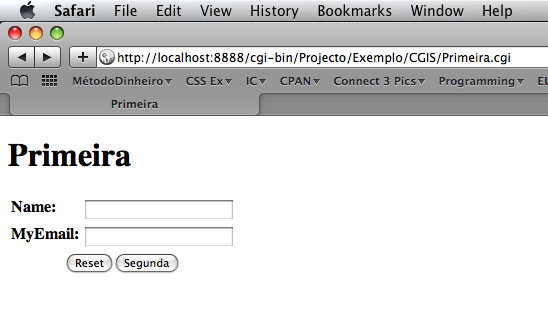
\includegraphics[width=0.7\textwidth]{./Images/Form.png}
\end{center}
\end{figure}

\vspace{.2cm}

Para além de transição directa, este é o tipo de transição mais simples que o DRAW suporta. Veremos tipos mais estruturados adiante.\\

\begin{small}
\textbf{Propriedades dos Campos}\\
\end{small}

\hspace{1cm}É usual, nos tempos de hoje, nem todos os campos de um formulário serem necessários para este ser submetido com sucesso.
Através de um dígito de sinalização o DRAW consegue interpretar se o campo é ou não de teor obrigatório. Também a partir de um dígito de
sinalização, é possível definir itens transitivos entre \emph{CGIs}, isto é, um campo transitivo submetido na \emph{CGI} de origem
será automaticamente preenchido na totalidade dos formulários da \emph{CGI} de destino.\\

\textbf{Exemplo:}

\begin{small}
\begin{lstlisting}
Primeira -> Segunda =>
        Name:0:0;
        Nick:1;
        MyEmail:0:1
\end{lstlisting}
\end{small}

\vspace{.2cm}

Neste exemplo observamos três variáveis ou campos, seguidos dos respectivos dígitos de sinalização. A variável \emph{Name} não é
transitiva nem de preenchimento obrigatório. A variável \emph{Nick} é transitiva e por último a variável \emph{MyEmail} é apenas de
preenchimento obrigatório. O primeiro dígito representa sempre a transitividade da variável e o segundo a obrigatoriedade.\\

\begin{small}
\textbf{Criar Campos de Selecção}\\
\end{small}

\hspace{1cm}Na secção de declaração de variáveis demonstramos que era possível declarar variáveis do tipo de selecção, agora vamos
mostrar como se adicionam a um formulário.

\begin{center}
\emph{Nodo Origem —$>$ Nodo Destino $\Rightarrow$
        Campo1;
        Campo2;
        Campo3[Opções]}
\end{center}

\vspace{.2cm}
\textbf{Exemplo:}

\begin{small}
\begin{lstlisting}
String Name;
Email MyEmail;
Select Gender;

Primeira -> Segunda => Name; MyEmail; Gender[Male,Female]
\end{lstlisting}
\end{small}

\vspace{.2cm}

\begin{figure}[!ht]
\begin{center}
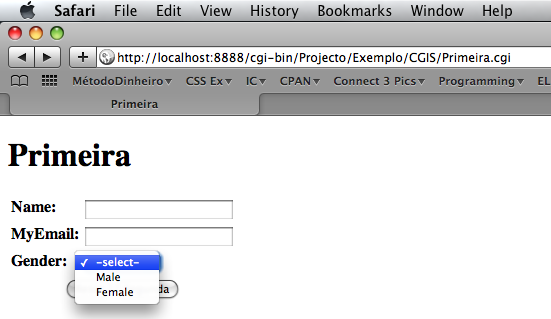
\includegraphics[width=0.7\textwidth]{./Images/Form2.png}
\end{center}
\end{figure}

\vspace{.2cm}

Um campo de selecção deve incluir todos os valores que pode assumir numa lista ladeada por parêntesis rectos ([]). O exemplo acima
demonstra uma caixa de selecção do género da pessoa, masculino ou feminino, de escolha obrigatória.\\

\begin{normalsize}
\textbf{Associar Funções a Transições}\\
\end{normalsize}

\hspace{1cm}Associar funções a transições funciona de maneira semelhante à sua declaração. Os tipos de dados de retorno são omitidos e
todos os outros tipos são substituídos por uma variável do mesmo tipo.\\

\textbf{Exemplo:}

\begin{small}
\begin{lstlisting}
WikiRepositorium;

text Description;
url Wikipage;
select Field;
select Conditions;
string Alias = test;
string Title;
string Keyword;
radio cs = 1;
string Theme;
int Relevance;

WikiRepositorium{
        vars searchEntry(string,int);
        List(string,string,url,text,string,int) removeAll(string,string,string,int);
}

Primeira -> Segunda =>
        Field[Alias,Title,Wikipage,Theme,Relevance];
        Conditions[StartWith,EndWith,Contains,Equal,NotEqual];
        cs[0,1];
        Keyword;
        (Alias,Title,Wikipage,Description,Theme,Relevance)
                                removeAll(Field,Keyword,Conditions,cs);
        searchEntry(Alias,cs)
\end{lstlisting}
\end{small}

\vspace{.2cm}

Com base na observação deste exemplo, podemos abordar quatro aspectos importantes.\\

\begin{small}
\textbf{Variáveis de Entrada e Retorno}\\
\end{small}

\hspace{1cm}Todas os tipos de dados são substituídos por uma variável do mesmo tipo e os tipos de retorno são omitidos, como já tinha
sido referido anteriormente, mas dê particular atenção à invocação da função \emph{removeAll}, ela encontra-se precedida por um tuplo
que contem algumas variáveis declaradas previamente no bloco de variáveis. Isto acontece porque o retorno dessa função é uma lista de
tuplos, sendo por isso necessário definir as variáveis às quais os valores de retorno dizem respeito. O mesmo acontece no caso do tipo de
retorno ser um único tuplo.\\

\begin{small}
\textbf{Consistência dos Dados}\\
\end{small}

\hspace{1cm}O DRAW quando interpreta a disposição do grafo, procura validar ao máximo a consistência dos dados inseridos pelo utilizador.
A invocação de funções não é excepção, por isso internamente, o DRAW efectua uma exaustiva comparação dos tipos de dados do protótipo da
função aos tipos de dados das variáveis que são definidas como parâmetros, tanto de entrada como saída.\\

\textbf{Exemplo:}

\begin{small}
\begin{lstlisting}
...
String Alias;

WikiRepositorium{
        vars searchEntry(string,int);
        List(int,string,url,text,string,int) removeAll(string,string,string,int);
}

Primeira -> Segunda =>
        ...
        (Alias,Title,Wikipage,Description,Theme,Relevance)
                                removeAll(Field,Keyword,Conditions,cs);
        ...
\end{lstlisting}
\end{small}

\vspace{.2cm}

No exemplo acima, ocorreria um erro ao compilar o projecto, visto que a variável \emph{Alias}, do tipo \emph{String}, é utilizada como
parâmetro de saída na função \emph{removeAll}, na posição de um parâmetro do tipo \emph{Int}, de acordo com o protótipo da função.
Existem algumas casos especiais que são excepção a esta regra como veremos mais à frente.
O erro gerado seria o seguinte:
                               
\begin{center}
\begin{small}
\emph{$"$Type mismatch! Variable: Alias, Function: removeAll, From Primeira to Segunda!$"$}
\end{small}
\end{center}

\begin{small}
\textbf{Parâmetros Previamente Inicializados}\\
\end{small}

\hspace{1cm}Variáveis previamente inicializadas no bloco de variáveis são também aceites como parâmetro de entrada de funções, isto
porque o DRAW encarrega-se de verificar se essa variável se encontra inicializada no caso de não ter sido submetida e não ser de
preenchimento obrigatório.\\

\textbf{Exemplo:}

\begin{small}
\begin{lstlisting}
string Alias = test;
radio cs;

WikiRepositorium{
        vars searchEntry(string,int);
}

Primeira -> Segunda =>
        cs[0,1];
        searchEntry(Alias,cs)
\end{lstlisting}
\end{small}

\vspace{.2cm}

Neste caso, a função \emph{searchEntry} iria receber como parâmetros a palavra $"$test$"$ e o valor submetido no campo \emph{cs}, isto
porque, como podemos observar, a variável \emph{Alias} não é utilizada no formulário do nodo \emph{Primeira} para o nodo \emph{Segunda},
logo assume o valor anteriormente atribuído pelo utilizador.\\

\begin{small}
\textbf{Campos Seleccionáveis}\\
\end{small}

\hspace{1cm}Por último, podemos observar no exemplo anterior que a variável \emph{cs} é do tipo \emph{Radio}, mas a função
\emph{searchEntry} recebe como parâmetros uma \emph{String} e um \emph{Int}, isto não era suposto dar erro? Não, porque, como referimos
acima, existem casos de excepção, mais propriamente os tipos de dados de selecção. Os tipos de selecção podem assumir qualquer outro tipo
logo são ignorados na verificação efectuada pelo DRAW, isto é, podem assumir qualquer tipo de dados de entrada sem que o DRAW lance um
erro para o saída.\\

\begin{normalsize}
\textbf{Invocar Objectos}\\
\end{normalsize}

\hspace{1cm}Para além de funções, também temos a possibilidade de invocar métodos no decorrer das travessias entre nodos. Para tal é
necessário existir pelo menos um objecto declarado no bloco de variáveis. Para definirmos um método, primeiro é crucial identificar o
objecto ao qual pertence, isso é possível das seguintes formas:\\

\begin{itemize}
        \item \emph{Objecto\{Método\}}
        \item \emph{Objecto\{Método(Parâmetros)\}}
        \item \emph{Objecto\{Módulo —$>$ Método\}}
        \item \emph{Objecto\{Módulo —$>$ Método(Parâmetros)\}}
\end{itemize}

Os métodos não precisam de ser previamente declarados no bloco de funções dado que na definição do objecto já é induzido o respectivo
módulo.\\

\begin{small}
\textbf{Inicializar Objectos}\\
\end{small}

\hspace{1cm}Um objecto antes de ser considerado apto para ser utilizado deve ser previamente criado e inicializado, em caso disso,
evitando assim erros em tempo de execução.\\

\textbf{Exemplo:}

\begin{small}
\begin{lstlisting}
string Alias = test;
radio cs;
Perl CGI MyObj;

WikiRepositorium{
        vars searchEntry(string,int);
}

Primeira -> Segunda =>
        cs[0,1];
        MyObj{CGI -> new};
        searchEntry(Alias,cs)
\end{lstlisting}
\end{small}

\vspace{.2cm}

No exemplo acima apresentado, declaramos um objecto denominado de \emph{MyObj}, pertencente ao módulo \emph{CGI} de \emph{Perl}.
Na travessia do nodo \emph{Primeira} para o nodo \emph{Segunda} é definido e invocado o método \emph{new} relativo ao mesmo objecto, isto
vai permitir que o objecto seja criado durante essa transição e que possa vir a ser utilizado posteriormente sem qualquer tipo de
problemas.\\

\textbf{Nota:} O estado dos diversos objectos é armazenado numa base de dados criada unicamente com o intuito de armazenar todos os
objectos utilizados numa determinada aplicação.\\

\begin{small}
\textbf{Invocar Métodos}\\
\end{small}

\hspace{1cm}No exemplo seguinte observamos algumas declarações de métodos que deverão executar durante as travessias pelo grafo
representado. São criados dois objectos, um \emph{CGI} e outro \emph{Data::Dumper}, ambos partilham \emph{Perl} como linguagem.
Transitando do nodo \emph{Primeira} para o \emph{Segunda}, os objectos são criados e os seus estados são armazenados numa base de dados
auxiliar. Se for feita a travessia contrária, serão invocados os métodos \emph{h3} e \emph{Dumper} dos objectos \emph{MyObj} e
\emph{ShObj} respectivamente. Os métodos são executados da mesma forma que as funções, excepto que o resultado final do objecto é
sempre armazenado numa base de dados para posterior acesso.\\

\textbf{Exemplo:}

\begin{small}
\begin{lstlisting}
string Alias = test;
radio cs;
Perl CGI MyObj;
Perl Data::Dumper ShObj;

Primeira -> Segunda =>
        MyObj{CGI -> new};
        ShObj{Data::Dumper -> new}
Segunda -> Primeira =>
        cs[0,1];
        MyObj{h3(Alias,cs)};
        ShObj{Dumper(Alias)}
\end{lstlisting}
\end{small}

\vspace{.2cm}

\begin{large}
\textbf{\emph{CSS}}\\
\end{large}

\hspace{1cm}O DRAW de raiz não aplica qualquer tipo de alteração à disposição das \emph{CGIs}, nem ao \emph{layout} final das páginas,
mas suporta a inserção de \emph{CSS} e presta uma pequena assistência em caso de se desejar alterar os elementos \emph{html} existentes
nas \emph{CGIs}. Veremos como nos seguintes tópicos.\\

\begin{normalsize}
\textbf{Munir um Projecto de \emph{CSS}}\\
\end{normalsize}

\hspace{1cm}Como já foi referido na secção das \emph{flags}, um projecto pode ser munido de \emph{CSS} através da \emph{flag DRAW\_CSS}.

\begin{center}
\begin{small}
\emph{DRAW\_CSS = /mycss.css;}
\end{small}
\end{center}

\begin{normalsize}
\textbf{Classes Auxiliares}\\
\end{normalsize}

\hspace{1cm}Aos vários elementos \emph{html} gerados pelo DRAW, é associada uma classe para facilitar sua manipulação através de
\emph{CSS}, isto permite ao utilizador um maior controlo sobre o resultado final da sua aplicação e tanto mais, a possibilidade de
personalização das páginas que compõem a aplicação.\\

\begin{itemize}
        \item \emph{forms} - Esta classe abrange todos os formulários criados para uma determinada \emph{CGI}
        \item \emph{link} - Esta classe abrange todos as âncoras criadas para uma determinada \emph{CGI}
        \item \emph{info} - Esta classe abrange a informação fornecida pelas \emph{flags} \emph{DRAW\_AUTHOR},\\
        \emph{DRAW\_WEB} e \emph{DRAW\_EMAIL}
        \item \emph{colist} - Esta classe abrange o resultado da impressão do conteúdo de uma lista de tuplos
        \item \emph{comp} - Esta classe abrange o resultado da impressão do conteúdo de um tuplo
        \item \emph{hash} - Esta classe abrange o resultado da impressão do conteúdo de uma \emph{hash}
        \item \emph{misc} - Esta classe abrange o resultado da impressão do conteúdo de uma variável
        \item \emph{list} - Esta classe abrange o resultado da impressão do conteúdo de uma lista
\end{itemize}

\begin{normalsize}
\textbf{Personalizar Formulários}\\
\end{normalsize}

\hspace{1cm}Para personalizar formulários é necessário aceder aos elementos gerados pelo DRAW. Manipular a totalidade do formulário é
possível acedendo ao elemento com o \emph{id} desejado. Por exemplo, assumindo-se que existe uma \emph{CGI} \emph{MainPage}, para se
aceder ao formulário de submissão dessa \emph{CGI} deve-se seleccionar o elemento com o \emph{id=$"$MainPage.cgi\_body$"$}.

\begin{center}
\emph{id=$"$\underline{NomeDaCGI}.cgi\_body$"$}
\end{center}

\hspace{1cm}Se o que se pretende é manipular um campo de cada vez, então deve-se seleccionar o elemento com

\begin{center}
\emph{id=$"$\underline{NomeDaCGI}.cgi\_\underline{NomeDoCampo}\_field$"$}
\end{center}

\hspace{1cm}Para além destes exemplos também é possível manipular as tabelas, linhas, células, etiquetas, etc.\\

\begin{large}
\textbf{Base de Dados}\\
\end{large}

\begin{normalsize}
\textbf{Acessibilidade}\\
\end{normalsize}

\hspace{1cm}Só é possível a existência de base de dados nos casos em que a \emph{flag} DRAW\_DB\_PATH se encontra definida, visto que
esta \emph{flag} indica o local onde a base de dados será criada, permitindo assim que um módulo com as rotinas de acesso seja instalado,
para posterior uso por parte da aplicação.

\begin{center}
\begin{small}
\emph{DRAW\_DB\_PATH = /Applications/MAMP/cgi-bin/Projecto/WikiRepositorium/Data/mydb.db;}
\end{small}
\end{center}

\begin{normalsize}
\textbf{Importar o Módulo}\\
\end{normalsize}

\hspace{1cm}Normalmente o módulo seria importado no bloco de funções, mas não aconselhamos essa prática devido ao facto de ser
preferível criar um novo módulo que o importe, isto porque, garante ao utilizador uma maior liberdade e adaptação aquando a criação de
uma determinada aplicação. Deste modo o utilizador pode adaptar e personalizar as mensagens de erro, o \emph{output} da aplicação, etc.
O módulo gerado pelo DRAW recebe o nome do título do projecto, originando assim um conflito no caso da criação de dois projectos com o
mesmo nome.\\

\textbf{Nota:} O módulo é compilado e instalado automaticamente pelo DRAW.\\

\begin{normalsize}
\textbf{Manipulação dos Dados}\\
\end{normalsize}

\hspace{1cm}Importar as funções de acesso à base de dados no DRAW é feito do mesmo modo que qualquer outra função. Numa fase inicial,
depois do módulo estar devidamente instalado, importam-se todas as funções que se pretende utilizar no bloco de funções, identificando
o(s) módulo(s) respectivo(s). Após as funções se encontrarem devidamente declaradas, basta definir as funções na representação do grafo
tal como foi apresentado anteriormente.\\

\textbf{Exemplo:}

\begin{small}
\begin{lstlisting}
BDACCESS;

Int Id;
String Name;
Int Age;
Email MyEmail;

BDACCESS{
        vars Select_Entry(int);
        void Insert_Entry(int,string,int,email);
}

Main -> Insert =>
        Id;
        Name;
        Age;
        MyEmail;
        Insert_Entry(Id,Name,Age,MyEmail)
Main -> Select =>
        Id;
        Select_Entry(Id)
Insert -> Main
Select -> Main
\end{lstlisting}
\end{small}

\vspace{.2cm}

\begin{normalsize}
\textbf{Controlo de Erros}\\
\end{normalsize}

\hspace{1cm}Existem vários erros possíveis de ocorrer quando se efectua um acesso à base de dados, mas na maioria das vezes não haverá problema visto que o DRAW efectua a maioria das validações necessárias para que as operações funcionem correctamente, em caso de sucesso ou insucesso do pedido. Erros de inserção de dados, duplicação, valores inconsistentes, campos obrigatórios e remoção consistente dos dados são todos verificados e validados pelo DRAW.

\newpage
%%
% Secção
%%
\subsection{\large Resultados Obtidos}

\hspace{1cm}Depois de estudada a estrutura da aplicação, resta-nos agora ver como esta se comporta na prática. Como foi visto acima nós podemos definir classes e relações com o uso da nossa linguagem, então como primeiro exemplo vamos criar duas classes com uma relação simples entre elas.\\

\begin{small}
\begin{lstlisting}
Class Emissao (
        Cod_Emissao:int(3) [key],
        Cod_Destinatario:int(3),
        Assunto: Nomes,
        DataEmissao:date);

Class Entidade (
        Cod_Entidade:int(3) [key],
        Nome,
        Morada: [optional],
        Telefone: [optional],
        Email: [optional]);

Relation ( Entidade, Emissao: 1, * );
Renom Nomes = varchar;
\end{lstlisting}
\end{small}

\bigskip
\hspace{1cm}Depois de corrermos o {\em dreql} com este {\em input} temos o seguinte resultado (na realidade são vários mas para já vamos só ver este):\\

\begin{small}
\begin{lstlisting}
create table Emissao (
        Cod_Emissao int(3) NOT NULL,
        Cod_Destinatario int(3) NULL,
        Assunto varchar NULL,
        DataEmissao date NULL,
        Cod_Entidade int(3) NOT NULL,
        primary key (Cod_Emissao),
        foreign key (Cod_Entidade) references Entidade(Cod_Entidade)
        );

create table Entidade (
        Cod_Entidade int(3) NOT NULL,
        Nome varchar(255),
        Morada varchar(255) NOT NULL,
        Telefone varchar(255) NOT NULL,
        Email varchar(255) NOT NULL,
        primary key (Cod_Entidade)
        );
\end{lstlisting}
\end{small}

\bigskip
\hspace{1cm}Acima podemos ver então a forma como são criadas as chaves com base nas relações que cada classe tem, neste exemplo ficamos com uma chave estrangeira na tabela 'Emissao' que faz referência à tabela 'Entidade'. Também podemos visualizar a forma como cada campo é definido dependendo das suas opções, por exemplo, o campo 'Morada' tem simplesmente a opção para o campo não ser opcional, no resultado {\em SQL} foi-lhe então atribuído a opção {\em NOT NULL} e o tipo de dados {\em varchar} com um tamanho predefenido, como já tinhamos explicado anteriormente.

\hspace{1cm}Agora vamos ver o que acontece caso tenhamos duas classes mas uma delas abstracta e outra que herda o conteúdo desta. Abaixo podemos ver as classes e o resultado depois da execução.\\

\begin{small}
\begin{lstlisting}
Abstract Grande (
        Coisas,
        Coisas_,
        Coisas__);

Class Controlo Extends Grande (
        Responsavel,
        Aprovacao:boolean,
        Cod_Controlo:int(3) [key]);
\end{lstlisting}
\end{small}

\begin{small}
\begin{lstlisting}
create table Controlo (
        Responsavel varchar(255) NULL,
        Aprovacao boolean,
        Cod_Controlo int(3) NOT NULL,
        Coisas varchar(255) NULL,
        Coisas_ varchar(255) NULL,
        Coisas__ varchar(255) NULL,
        primary key (Cod_Controlo),
        );
\end{lstlisting}
\end{small}

\bigskip
\hspace{1cm}Como podemos visualizar, a tabela 'Controlo' herdou todos os campos da classe abstracta que por sua vez não aparece no modelo relacional, como é de esperar.

\hspace{1cm}No próximo teste vamos acrescentar um tipo de dados composto, neste caso o {\em set}, e ver como se comporta.\\

\begin{small}
\begin{lstlisting}
Class Registo (
        Cod_Registo:int(3) [key],
        TipoRegisto: Set,
        DataRegisto:date);
\end{lstlisting}
\end{small}

\begin{small}
\begin{lstlisting}
create table Registo (
        Cod_Registo int(3) NOT NULL,
        DataRegisto date NULL,
        primary key (Cod_Registo)
        );

create table Registo_TipoRegisto (
        TipoRegisto varchar(255) NULL,
        Cod_Registo int(3) NOT NULL,
        primary key (TipoRegisto, Cod_Registo),
        foreign key (Cod_Registo) references Registo(Cod_Registo)
        );
\end{lstlisting}
\end{small}

\bigskip
\hspace{1cm}Este tipo de dados composto dá origem a uma nova tabela que mantêm uma relação com a tabela onde o campo respectivo estava definido. A nova tabela recebe como chave estrangeira a chave primária da tabela original e como chave primária o campo que tinha {\em set} como tipo de dados.

\hspace{1cm}Mas estes resultados não são os únicos que o {\em dreql} retorna, além destes são também geradas as funções que integram o {\em CRUD} sendo estas diferentes para cada tabela. Abaixo mostramos o exemplo da função de remoção para a tabela 'Registo', como é óbvio não vamos mostrar todas já que são funções com dimensões bastante razoáveis.\\

\begin{small}
\begin{lstlisting}
sub delete_Registo {
   my $condition = shift;
   my $dbh = DBI->connect("dbi:SQLite:dbname=[DATABASE_PATH]"
      ,"[DB_USERNAME]","[DB_PASSWORD]",
      { RaiseError => 1, AutoCommit => 0, unicode => 1 })
      or die $DBI::errstr;

   foreach ( keys %{$db->{Registo}->{'primkeys'}} ) {
      foreach my $tb ( keys %{$db} ) {
         if ( exists $db->{$tb}->{'fgnkeys'}->{$_} ) {
            my $notnull = 0;
            foreach my $opt ( @{$db->{$tb}->{'fields'}->{$_}->{'options'}} ) {
               if ( $opt =~ /\boptional\b/i ) { $notnull = 1; last }
               else { next }
            }
            unless ( 1 == $notnull ) {
               my $sql;
               if ( 'undef' eq $condition ) { $sql = "SELECT $_ FROM Registo" }
               else { $sql = "SELECT $_ FROM Registo WHERE $condition" }
               my $sth = $dbh->prepare($sql) or $@ = $dbh->errstr;
               $sth->execute or $@ = $dbh->errstr;
               my $rv = $sth->fetchall_hashref($_);
               foreach my $key ( keys %{$rv} ) {
                  my $sql = "UPDATE $tb SET $_=? WHERE $_=$key";
                  my $sth = $dbh->prepare($sql) or $@ = $dbh->errstr;
                  $sth->execute(undef) or $@ = $dbh->errstr;
               }
               $dbh->commit
            }
         }
      }
   }
   my $sql;
   if ( 'undef' eq $condition ) { $sql = "DELETE FROM Registo" }
   else { $sql = "DELETE FROM Registo WHERE $condition" }
   my $sth = $dbh->prepare($sql) or $@ = $dbh->errstr;
   my $res=$sth->execute or $@ = $dbh->errstr;
   $dbh->commit;
   $dbh->disconnect or warn $dbh->errstr;
   return $res;
}
\end{lstlisting}
\end{small}

\bigskip
\hspace{1cm}Nos anexos B e C temos a totalidade do ficheiro de entrada e o resultado obtido, respectivamente, depois de terminado o processamento.

\newpage

%%
% Secção - Conclusão
%%

%Síntese / Recapitulação do Relatório
%Resultado Atingido / Crítica
%Trabalho Futuro

\newpage
\section{\LARGE Conclusão}

\hspace{1cm}Durante este relatório vimos as várias camadas que dividem a aplicação, mostramos como a linguagem que desenvolvemos faz a representação de um modelo de classes e como este é posteriormente convertido para um modelo relacional ({\em dreql}) para podermos criar a base de dados. Vimos também como o {\em dreql} gera o código para as funções que são incorporadas no {\em CRUD} de forma a mais tarde serem utilizadas pelo {\em Draw}.

\hspace{1cm}Estudamos em detalhe a estrutura interna do {\em Draw} e nisto vimos como era aplicada a filosofia dos autómatos reactivos neste. Vimos várias propriedades do {\em Draw} e a importância que estas têm no seu funcionamento e apresentamos várias alternativas para as mesmas.

\hspace{1cm}Conseguimos concluir tudo o que nos propusemos apresentar dentro da data estipulada, que podemos dizer já que foi mais que justa, já que tivemos acesso ao enunciado praticamente no início do ano lectivo e os professores foram bastante flexíveis nas datas (no nosso entender até demais). Se voltassemos a fazer este projecto, haveriam coisas que alteraríamos como por exemplo a forma como as relações estão definidas na nossa linguagem já que podiamos ter embebido esta informação no momento em que fazemos a descrição da classe. Na parte do {\em Draw} voltaríamos a fazer tudo sem nenhuma alteração, já que refizemos esta camada duas vezes.

\hspace{1cm}Como trabalho futuro, tendo em conta o {\em dreql}, estamos a pensar incluir novos tipos de dados compostos e novas opções, também estamos a pensar fazer algumas alterações à nossa linguagem. Isto se não fizermos a conversão total do código para {\em perl} que, para já, é a nossa primeira opção.

\hspace{1cm}Quanto ao {\em Draw}, para já estamos a pensar criar uma {\em makefile} em {\em perl} para o nosso projecto, mas depois estamos a pensar fazer alterações sérias à estrutura. Vamos tentar fazer com que seja possível importar as próprias classes me {\em Java} utilizando o módulo {\em Java::Import} do {\em perl}. Também vamos tentar fazer com que a aplicação suporte diferentes motores para bases de dados (para já só suporta {\em SQLite}) para que seja possível o utilizador utilizar as tecnologias em que se sente mais à vontade.

\hspace{1cm}Quanto ao grafo que define a aplicação, estamos a pensar convertê-lo para uma representação em {\em XML}\useglosentry{glos:XML} criar um {\em XML schema}\footnote{{\em http://en.wikipedia.org/wiki/XML\_schema}} para estes. Este é uma alteração que não foi pensada com o objectivo de algum ganho em eficiência mas sim pela legibilidade e manutenção.

\hspace{1cm}Também estamos a pensar fazer umas melhorias no campo da segurança, incluíndo {\em md5}\footnote{{\em http://en.wikipedia.org/wiki/MD5}} na codificação das {\em passwords} dos utilizadores de forma a tornar a tornar esta aplicação o mais perto do real possível. Não queremos com este projecto simplesmente uma nota porque nós estamos interessados em não o deixar morrer e trabalhar nele de forma a cumprirmos todos estes objectivos que propusemos aqui.

\newpage

\begin{appendix}
\section{Gramática}
\begin{small}
\begin{lstlisting}
dreql   :       commands
                -> ^(DREQL commands)
        ;

commands        :       (command ';')+
                -> ^(COMMANDS command+)
        ;

command :       (a=dclass | b=relation | c=renom)
                -> {a!=null}? ^(COMMAND dclass)
                -> {b!=null}? ^(COMMAND relation)
                -> ^(COMMAND renom)
        ;

dclass  : ('class' | 'Class') table '(' fields ')'
          -> ^(CLASS table fields)
          | ('abstract' | 'Abstract') table '(' fields ')'
          -> ^(ABSTRACT table fields)
          | ('class' | 'Class') table ('extends' | 'Extends') table '(' fields ')'
          -> ^(EXTENDS table table fields)
        ;

relation        :
   ('relation' | 'Relation') '(' table ',' table ':' reltype ',' reltype ')'
                -> ^(RELATION table table reltype reltype)
        ;

renom   :       ('renom' | 'Renom') TYPE '=' TYPE
                -> ^(RENOM TYPE TYPE)
        ;

table   :       TYPE
                -> ^(TABLE TYPE)
        ;

fields  :       field (',' field)*
                -> ^(FIELDS field+)
        ;

field   :       fieldname ':' datatype '[' optional ']'
                -> ^(FIELD fieldname datatype optional)
                | fieldname ':'  '[' optional ']'
                -> ^(FIELD fieldname optional)
                | fieldname ':' datatype
                -> ^(FIELD fieldname datatype)
                | fieldname
                -> ^(FIELD fieldname)
        ;

fieldname       :       TYPE
                -> ^(FIELDNAME TYPE)
        ;


optional        :       option (',' option)*
                -> ^(OPTIONAL option+)
        ;
datatype        :       TYPE '(' NUM ')'
                -> ^(DATATYPE TYPE NUM)
                | TYPE
                -> ^(DATATYPE TYPE)
                | ('enum' | 'Enum') '(' enumopt ')'
                -> ^(DATATYPE ENUM enumopt)
                | set
                -> ^(DATATYPE set)
        ;

set     :       ('set' | 'Set') TYPE '(' NUM ')'
                -> ^(SETTYPE TYPE NUM)
                | ('set' | 'Set') TYPE
                -> ^(SETTYPE TYPE)
                | ('set' | 'Set')
                -> ^(SETTYPE SET)
        ;

enumopt :       args (',' args)*
                -> ^(ENUMOPT args+)
        ;

args    :       VAL
                -> ^(ARGS VAL)
        ;

option  :
   (a='editable' | b='visible' | c='optional' | d='masked' | e='key' | 'autoinc')
                -> {a!=null}? ^(OPTION EDITABLE)
                -> {b!=null}? ^(OPTION VISIBLE)
                -> {c!=null}? ^(OPTION OPTIONAL)
                -> {d!=null}? ^(OPTION MASKED)
                -> {e!=null}? ^(OPTION KEY)
                -> ^(OPTION AUTOINC)
        ;

reltype :
   (a='1' | b='0..1' | c='1..*' | d='0..*' | e='*' | f=NUM | NUM '..' NUM)
                -> {a!=null}? ^(RELTYPE ONE)
                -> {b!=null}? ^(RELTYPE ZEROTOONE)
                -> {c!=null}? ^(RELTYPE ONETON)
                -> {d!=null}? ^(RELTYPE ZEROTON)
                -> {e!=null}? ^(RELTYPE NTOM)
                -> {f!=null}? ^(RELTYPE NUM)
                -> ^(RELTYPE NUM NUM)
        ;

NUM     :       ('0'..'9')+
        ;

TYPE    :       ('A'..'Z' | 'a'..'z' | '_')+
        ;

VAL     :       ('\'' (options{greedy=false;}:.)*  '\'')
        ;

NS      :       (' ' | '\t' | '\n' | 'r') { skip(); }
        ;

COMMENT :       '/*' (options {greedy=false; }:.)* '*/' { skip(); }
        ;

LINE_COMMENT      :        '//' ~('\n'|'\r')* '\r'? '\n' { skip(); }
        ;
\end{lstlisting}
\end{small}

\newpage

\section{Modelo de Classes}
\begin{small}
\begin{lstlisting}
Abstract Grande (
        Coisas,
        Coisas_,
        Coisas__);
Class Registo (
        Cod_Registo:int(3) [key],
        TipoRegisto: Set,
        DataRegisto:date);
Class Controlo Extends Grande (
        Responsavel,
        Aprovacao:boolean,
        Cod_Controlo:int(3) [key] );
Class Recepcao (
        Cod_Recepcao:int(3) [key],
        Cod_Remetente:int(3) ,
        Assunto: Nomes,
        DataRecepcao:date);
Class Emissao (
        Cod_Emissao:int(3) [key],
        Cod_Destinatario:int(3),
        Assunto: Nomes,
        DataEmissao:date);
Class Entidade (
        Cod_Entidade:int(3) [key],
        Nome,
        Morada: [optional],
        Telefone: [optional],
        Email: [optional]);
Relation ( Registo, Emissao: 1, * );
Relation ( Registo, Controlo: 1, 1 );
Relation ( Registo, Recepcao: 1, *);
Relation ( Entidade, Emissao: 1, * );
Relation ( Entidade, Recepcao: 1, * );
Renom Nomes = varchar;
\end{lstlisting}
\end{small}

\newpage

\section{Modelo Relacional}
\begin{small}
\begin{lstlisting}
create table Registo_TipoRegisto (
        TipoRegisto varchar(255) NULL,
        Cod_Registo int(3) NOT NULL,
        primary key (TipoRegisto, Cod_Registo),
        foreign key (Cod_Registo) references Registo(Cod_Registo)
        );
create table Controlo (
        Responsavel varchar(255) NULL,
        Aprovacao boolean,
        Cod_Controlo int(3) NOT NULL,
        Coisas varchar(255) NULL,
        Coisas_ varchar(255) NULL,
        Coisas__ varchar(255) NULL,
        Cod_Registo int(3) NOT NULL,
        primary key (Cod_Controlo),
        foreign key (Cod_Registo) references Registo(Cod_Registo)
        );
create table Emissao (
        Cod_Emissao int(3) NOT NULL,
        Cod_Destinatario int(3) NULL,
        Assunto varchar NULL,
        DataEmissao date NULL,
        Cod_Registo int(3) NOT NULL,
        Cod_Entidade int(3) NOT NULL,
        primary key (Cod_Emissao),
        foreign key (Cod_Registo) references Registo(Cod_Registo),
        foreign key (Cod_Entidade) references Entidade(Cod_Entidade)
        );
create table Recepcao (
        Cod_Recepcao int(3) NOT NULL,
        Cod_Remetente int(3) NULL,
        Assunto varchar NULL,
        DataRecepcao date NULL,
        Cod_Registo int(3) NOT NULL,
        Cod_Entidade int(3) NOT NULL,
        primary key (Cod_Recepcao),
        foreign key (Cod_Registo) references Registo(Cod_Registo),
        foreign key (Cod_Entidade) references Entidade(Cod_Entidade)
        );
create table Registo (
        Cod_Registo int(3) NOT NULL,
        DataRegisto date NULL,
        primary key (Cod_Registo)
        );
create table Entidade (
        Cod_Entidade int(3) NOT NULL,
        Nome varchar(255),
        Morada varchar(255) NOT NULL,
        Telefone varchar(255) NOT NULL,
        Email varchar(255) NOT NULL,
        primary key (Cod_Entidade)
        );
\end{lstlisting}
\end{small}

% \newpage
% \section{}
% \begin{small}
% \begin{lstlisting}
% \end{lstlisting}
% \end{small}

\end{appendix}

\newpage

\printglossary
\addcontentsline{toc}{section}{\LARGE Glossary}

\end{document}